\begin{SCn}

\scnsectionheader{\currentname}

\scnstartsubstruct

\scnheader{Предметная область темпоральных сущностей}
\scnidtf{Предметная область темпоральных связей и отношений}
\scnidtf{Предметная область временных сущностей}
\scniselement{предметная область}
\scnsdmainclasssingle{временная сущность}
\scnsdclass{прошлая сущность;настоящая сущность;будущая сущность;временная связь;ситуация;процесс;процесс в sc-памяти;процесс во внешней среде ostis-системы;материальная сущность;воздействие;отношение;класс временных связей;класс временных и постоянных связей;множество;ситуативное множество;неситуативное множество;частично ситуативное множество;темпоральная связь;темпоральное отношение;начало\scnsupergroupsign;завершение\scnsupergroupsign;длительность\scnsupergroupsign;тысячелетие;век;год;месяц;сутки;час;минута;секунда}
\scnsdrelation{воздействующая сущность*;объект воздействия*;начальная ситуация*;причинная ситуация*;конечная ситуация*;событие*;последний добавленный sc-элемент\scnrolesign;темпоральное включение*;темпоральная часть*;начальный этап*;конечный этап*;промежуточный этап*;темпоральное включение без совпадения начальных и конечных моментов*;темпоральное включение с совпадением начальных моментов*;темпоральное включение с совпадением конечных моментов*;темпоральное совпадение*;темпоральное объединение*;темпоральная декомпозиция*;темпоральная смежность*;темпоральная последовательность с промежутком*;темпоральная последовательность с пересечением*;номер тысячелетия\scnrolesign;номер века\scnrolesign;номер года\scnrolesign;номер месяца в году\scnrolesign;номер суток в месяце\scnrolesign;номер часа в дне\scnrolesign;номер минуты в часе\scnrolesign;номер секунды в минуте\scnrolesign}

\scnheader{временная сущность}
\scnidtf{временно существующая сущность}
\scnidtf{нестационарная сущность}
\scnidtf{сущность, имеющая и/или начало, и/или конец своего существования}
\scnidtf{sc-элемент, являющийся знаком некоторой временно существующей сущности}
\scnidtf{сущность, обладающая темпоральными характеристиками (длительностью, начальным моментом, конечным моментом и т.д.)}
\scnsubdividing{прошлая сущность;настоящая сущность;будущая сущность}
\scnsubdividing{временная связь;темпоральная структура\\
	\scnaddlevel{1}
		\scnidtf{структура, содержащая хотя бы одну временную сущность}
		\scnrelfrom{включение}{структура}
		\scnnote{Следует отличать:
			\begin{scnitemize}
				\item временный характер самой структуры как sc-элемента;
				\item временный характер sc-элементов, принадлежащих данной структуре, и сущностей, обозначаемых этими sc-элементами;
				\item временный характер пар принадлежности, связывающих структуру с ее элементами.
			\end{scnitemize}}
		\scnidtf{структура, описывающая темпоральные свойства (свойства, связанные со временем) окружающей среды, частью которой являются также и различные базы знаний кибернетических систем (в том числе и собственная база знаний).}
		\scnsubdividing{ситуация\\
			\scnaddlevel{1}
				\scnidtf{статическая темпоральная структура}
			\scnaddlevel{-1}
			;процесс\\
			\scnaddlevel{1}
				\scnidtf{динамическая структура}
				\scnidtf{динамическая темпоральная структура}
			\scnaddlevel{-1}}
	\scnaddlevel{-1}
	;материальная сущность}
\scnsubdividing{непрерывная временная сущность\\
	\scnaddlevel{1}
	\scnsubdividing{точечная временная сущность\\
		\scnaddlevel{1}
			\scnidtf{атомарная временная сущность}
			\scnidtf{условно мгновенная временная сущность}
			\scnidtf{временная сущность, длительность существования которой в данном контексте считается несущественной (пренебрежительно малой)}
		\scnaddlevel{-1}
		;длительная непрерывная временная сущность}
	\scnaddlevel{-1}	
	;дискретная временная сущность\\
	\scnaddlevel{1}
	\scnidtf{временная сущность, которая может быть декомпозирована на последовательность точечных временных сущностей}
	\scnidtf{временная сущность, которой соответствует некоторый временной ряд параметров (состояний) точечных временных сущностей, на которые декомпозируется исходная временная сущность}
	\scnaddlevel{-1}	
	;прерывистая временная сущность\\
	\scnaddlevel{1}
	\scnidtf{временная сущность, являющаяся результатом соединения нескольких не только точечных временных сущностей}
	\scnidtf{временная сущность с прерываниями}
	\scnaddlevel{-1}
}
\scnaddlevel{1}
	\scnnote{Следует отметить, что приведенная классификация \textit{временных сущностей} характеризует не столько сами \textit{временные сущности}, сколько наши знания о них и степень детализации знаний об этих сущностях, с которой они описаны в базе знаний. Так, если для решения конкретных задач не важно, как изменялась некоторая \textit{временная сущность} в рамках какого-либо периода времени, а важно только ее начальное и конечное состояние, то она может рассматриваться как \textit{точечная временная сущность}. Впоследствии же та же \textit{временная сущность} может быть рассмотрена и описана с большей степенью детализации, и таким образом, уже не будет точечной.}
\scnaddlevel{-1}
\scnexplanation{Следует отличать:
\begin{scnitemize}
    \item временный характер сущности, обозначаемой \textit{sc-элементом};
    \item временный характер существования самого \textit{sc-элемента} в рамках \textit{sc-памяти}, поскольку в ходе обработки информации каждый \textit{sc-элемент} может быть удален из \textit{sc-памяти}; 
    \item временный характер описываемых ситуаций, событий и самих процессов;
    \item временный характер хранения в sc-памяти тех sc-конструкций, которые являются самими описаниями соответствующих ситуаций, событий и процессов.
\end{scnitemize}
}

\scnheader{следует отличать*}
\scnhaselementset{временная сущность;процесс}
\scnnote{Следует отличать, например, \textit{материальную сущность} (некоторый физический или, в частности, биологический объект) от различных динамических структур (\textit{процессов}), которые с той или иной степенью детализации и в том или ином ракурсе отражают (описывают) динамику изменений этой \textit{материальной сущности}. 

При этом сам \textit{процесс} как уточнение динамики некоторой последовательности ситуаций и событий, также является сущностью, принадлежащей к классу \textit{временных сущностей}.}

\scnheader{прошлая сущность}
\scnidtf{сущность, существовавшая в прошлом времени}
\scnidtf{сущность прошлого времени}
\scnidtf{сущность, завершившая свое существование}

\scnheader{настоящая сущность}
\scnidtf{сущность, существующая в текущий момент времени}
\scnidtf{сущность, существующая сейчас}
\scnidtf{сущность настоящего времени}

\scnheader{будущая сущность}
\scnidtf{возможно будущая сущность}
\scnidtf{прогнозируемая временная сущность}
\scnidtf{временная сущность, которая может существовать в будущем}
\scnidtf{сущность, которая может или должна начать свое существование в будущем времени}
\scnrelfrom{включение}{инициированное действие}
\scnexplanation{Каждой \textbf{\textit{будущей сущности}} можно поставить в соответствие вероятность ее возникновения.}

\scnheader{временная связь}
\scnidtf{нестационарная связь}
\scnidtf{временно существующая связь}
\scnexplanation{Каждая \textbf{\textit{временная связь}} представляет собой \textit{связку}, принадлежащую множеству \textit{временных сущностей}.

Понятие \textbf{\textit{временной связи}} не следует путать с понятием \textit{темпоральной связи}, которая сама является \textit{постоянной сущностью}, описывающей то, как связаны во времени некоторые \textit{временные сущности}.
}

\scnheader{ситуация}
\scnidtf{состояние}
\scnidtf{временная структура}
\scnidtf{временно существующая структура}
\scnidtf{квазистационарная структура}
\scnidtf{состояние некоторой динамической системы, описываемое с некоторой степенью детализации (подробности)}
\scnidtf{квазистационарная структура, существующая временно (в течение некоторого отрезка времени)}
\scnexplanation{Под ситуацией понимается \textit{структура}, содержащая, по крайней мере, один элемент, который является \textit{временной сущностью}. Наличие в рамках ситуации нескольких \textit{временных сущностей} говорит о том, что существует момент времени (в прошлом, настоящем или будущем), в который все они существуют одновременно.}

\scnheader{процесс}
\scnidtf{процесс преобразования некоторой временной сущности из одного состояния в другое}
\scnidtf{процесс перехода от одной ситуации к другой}
\scnidtf{абстрактный процесс}
\scnidtf{информационная модель некоторых преобразований}
\scnidtf{динамическая sc-модель}
\scnidtf{динамическая структура}
\scnrelfrom{включение}{воздействие}
\scnexplanation{Каждый \textbf{\textit{процесс}} определяется (задается) либо возникновением или исчезновением связей, связывающих заданную \textit{временную сущность} с другими сущностями, либо возникновением или исчезновением связей, связывающих части указанной \textit{временной сущности} с другими сущностями. 

Многим \textbf{\textit{процессам}} можно поставить в соответствие \textit{ситуацию}, которая является его \textit{начальной ситуацией*} и \textit{ситуацию}, которая является его \textit{конечной ситуацией*}, то есть указать \textit{ситуации}, переход между которыми осуществляется в ходе \textbf{\textit{процесса}}.

При этом знаки тех \textit{временных сущностей}, с которыми связаны изменения, описываемые некоторым \textbf{\textit{процессом}}, входят в данный \textbf{\textit{процесс}} как элементы и при необходимости уточняются дополнительными \textit{ролевыми отношениями}.}
\scnsubdividing{процесс в sc-памяти;процесс во внешней среде ostis-системы}
\scnnote{Каждой \textbf{\textit{материальной сущности}} можно поставить в соответствие различные \textit{процессы}, описывающие ее преобразование из одного состояния в другое.}
\scnnote{Поскольку \textit{процесс} представляет собой изменяющуюся во времени динамическую структуру, то полностью представить процесс в базе знаний в общем случае не представляется возможным. Однако, можно ввести sc-элемент, обозначающий конкретный процесс, с необходимой степенью детализации описать его декомпозицию на более частные подпроцессы и/или описать ситуации, соответствующие состояниям процесса в разные моменты времени. В данном случае можно провести некоторую аналогию с \textit{бесконечными множествами}, все элементы которых физически не могут быть представлены в базе знаний одновременно, тем не менее, само множество и некоторые из его элементов могут быть описаны с необходимой степенью детализации.}

\scnheader{воздействие}
\scnidtf{процесс, осуществляющийся на основе (в результате) воздействия одной сущности на другую}
\scnrelfrom{включение}{действие}
\scnexplanation{Каждому \textbf{\textit{воздействию}} может быть поставлена в соответствие (1) некоторая \textit{воздействующая сущность*}, т.е. сущность, осуществляющая \textbf{\textit{воздействие}} (в частности, это может быть некоторое физическое поле), и (2) некоторый \textit{объект воздействия*}, т.е. сущность, на которую воздействие направлено. Если \textbf{\textit{воздействие}} связано с \textit{материальной сущностью}, то его объектом воздействия является либо сама эта \textit{материальная сущность}, либо некоторая ее пространственная часть.}

\scnheader{исходная ситуация*}
\scnidtf{начальная ситуация процесса*}
\scnidtf{начальная ситуация*}
\scniselement{бинарное отношение}
\scnrelfrom{первый домен}{процесс}
\scnrelfrom{второй домен}{ситуация}
\scnexplanation{Связки отношения \textbf{\textit{исходная ситуация*}} связывают некоторый \textit{процесс} и некоторую ситуацию, являющуюся начальной для этого \textit{процесса}, и, как правило, изменяемой в течение выполнения этого \textit{процесса}.

Первым компонентом каждой связки отношения \textbf{\textit{исходная ситуация*}} является знак \textit{процесса}, вторым -- знак начальной \textit{ситуации}.}

\scnheader{причинная ситуация*}
\scnsubset{начальная ситуация*}
\scnexplanation{Под причинной ситуацией понимается такая \textit{начальная ситуация*}, которая обладает достаточной полнотой для однозначного задания инициируемого \textit{процесса}.}

\scnheader{конечная ситуация*}
\scnidtf{конечная ситуация процесса*}
\scnidtf{результирующая ситуация*}
\scniselement{бинарное отношение}
\scnrelfrom{первый домен}{процесс}
\scnrelfrom{второй домен}{ситуация}
\scnexplanation{Связки отношения \textbf{\textit{конечная ситуация*}} связывают некоторый \textit{процесс} и некоторую \textit{ситуацию}, ставшую результатом выполнения этого \textit{процесса}, то есть его следствием.

Первым компонентом каждой связки отношения \textbf{\textit{конечная ситуация*}} является знак \textit{процесса}, вторым -- знак конечной \textit{ситуации}.}

\scnheader{точечный процесс}
\scnidtf{атомарный процесс}
\scnidtf{условно мгновенный процесс}
\scnidtf{процесс, длительность которого в данном контексте считается несущественной (пренебрежимо малой)}
\scnsubset{точечная временная сущность}

\scnheader{элементарный процесс}
\scnidtf{процесс, детализация которого на входящие в него подпроцессы в текущем контексте не производится}
\scnsuperset{точечный процесс}
\scnnote{Элементарные процессы могут иметь длительность и, следовательно, не обязательно являются атомарными процессами.}
\scnnote{Понятия \textit{точечного процесса} и \textit{элементарного процесса}, как и понятие \textit{точечной временной сущности} в целом, характеризуют не столько характеристики самого \textit{процесса}, сколько степень наших знаний о нем и степень детализации описания процесса в базе знаний. Так, очевидно, что любой процесс, протекающий в компьютерной системе, может быть при необходимости детализирован до уровня команд процессора, затем до уровня микропрограмм и даже до уровня физических процессов (изменения физических характеристик сигналов), однако чаще всего такая детализация не требуется.}
\scnaddlevel{1}
	\scnrelto{примечание}{точечный процесс}
\scnaddlevel{-1}

\scnheader{событие}
\scnsubset{точечная временная сущность}
\scnidtf{точечная временная сущность, являющаяся началом и/или завершением какой-либо временной сущности (например, процесса)}
\scnidtf{граничная точка временной сущности}
\scnrelfrom{описание примера}{
\scnfilescg{figures/sd_temp_entities/event.png}
}
\scnaddlevel{1}
	\scnnote{Одно и то же событие может быть одновременно завершением одной временной сущности и началом другой. В приведенном примере событие $\bm{ei}$ является завершением временной сущности $\bm{si}$ и началом временной сущности $\bm{sj}$.}
\scnaddlevel{-1}

\scnheader{начало*}
\scnidtf{быть начальным событием заданной временной сущности*}
\scnrelfrom{первый домен}{временная сущность}
\scnrelfrom{второй домен}{событие}
\scnidtf{быть начальной точечной временной частью заданной временной сущности*}

\scnheader{завершение*}
\scnidtf{конец*}
\scnidtf{быть конечным событием заданной временной сущности*}
\scnidtf{быть конечной точечной временной частью заданной временной сущности*}
\scnrelfrom{первый домен}{временная сущность}
\scnrelfrom{второй домен}{событие}

\scnheader{событие*}
\scniselement{бинарное отношение}
\scnexplanation{Связки отношения \textbf{\textit{событие*}} связывают знак процесса и ориентированную пару, первым компонентом которой является знак \textit{начальной ситуации*} данного процесса, вторым компонентом -- знак \textit{конечной ситуации*} данного процесса.}
\scnrelfrom{описание примера}{
\scnfilescg{figures/sd_temp_entities/nrel_event.png}
}

\scnheader{детализация процесса*}
\scnidtf{Бинарное ориентированное отношение, каждая связка которого связывает некоторый процесс с более детальным его описанием, что предполагает представление декомпозиции этого процесса на систему взаимосвязанных его подпроцессов (в том числе элементарных).}
\scnrelfrom{пример}{Переход от процесса, соответствующего какой-либо программе, к рассмотрению декомпозиции этого процесса (протокола) в терминах языка программирования высокого уровня, затем переход для каждого из полученных подпроцессов (операторов языка высокого уровня) к детализации выполнения этих подпроцессов на уровне машинных операций, выполняемых процессором компьютера (на уровне ассемблера), и далее к детализации выполнения подпроцессов уровня машинных операций к подпроцессам на уровне языка микропрограммирования. Таким образом, детализация процесса может быть иерархической, вплоть до уровня \textit{элементарных процессов}.}

\scnheader{отношение}
\scnsubdividing{класс временных связей;класс постоянных связей;класс временных и постоянных связей}

\scnheader{класс временных связей}
\scnidtf{отношение, все связки которого являются нестационарными}
\scnexplanation{В общем случае \textbf{\textit{класс временных связей}} не является \textit{ситуативным множеством}, поскольку факт принадлежности некоторой \textit{временной связи} такому классу следует считать постоянным, а не временным, поскольку временность/постоянство связи и ее семантический тип, задаваемый классом (отношением), это принципиально разные параметры (характеристики, признаки) любой связи.}

\scnheader{класс постоянных связей}
\scnidtf{отношение, все связки которого являются стационарными}

\scnheader{класс временных и постоянных связей}
\scnidtf{отношение, некоторые (но не все) связки которого являются нестационарными}

\scnheader{множество}
\scnsubdividing{ситуативное множество;неситуативное множество;частично ситуативное множество}

\scnheader{ситуативное множество}
\scnidtf{полностью ситуативное множество}
\scnexplanation{Под \textbf{\textit{ситуативным множеством}} понимается постоянное множество, у которого все выходящие из него связи принадлежности являются \textit{временными сущностями}.

В частности, ситуативное множество может использоваться как вспомогательная динамическая структура, которая содержит элементы некоторых структур, обрабатываемые в данный момент, например, это может быть копия некоторого множества, из которой постепенно удаляются элементы по мере их просмотра и обработки. В случае, когда такая структура содержит всего один элемент, ее можно считать \underline{указателем} на данный элемент, при этом в разные моменты времени это могут быть разные элементы.}

\scnheader{последний добавленный sc-элемент\scnrolesign}
\scniselement{ролевое отношение}

\scnheader{неситуативное множество}
\scnexplanation{Под \textbf{\textit{неситуативным множеством}} понимается постоянное множество, у которого все выходящие из него связи принадлежности являются \textit{постоянными сущностями}.}

\scnheader{частично ситуативное множество}
\scnexplanation{Под \textbf{\textit{частично ситуативным множеством}} понимается постоянное множество, у которого некоторые (но не все) выходящие из него связи принадлежности являются \textit{временными сущностями}.}

\scnheader{темпоральная связь}
\scnidtf{связь во времени}
\scnidtf{\uline{постоянная} связь, описывающая связь во времени между временными сущностями}

\scnheader{темпоральное отношение}
\scnrelto{семейство подмножеств}{темпоральная связь}
\scnidtf{класс темпоральных связей}
\scnidtf{отношение, задающее темпоральные связи между временными сущностями}
\scnhaselement{темпоральное включение*}
\scnhaselement{темпоральное объединение*}
\scnhaselement{темпоральная декомпозиция*}
\scnhaselement{темпоральная последовательность*}
\scnaddlevel{1}
\scnsubdividing{темпоральная смежность*;темпоральная последовательность с промежутком*;темпоральная последовательность с пересечением*}
\scnaddlevel{-1}

\scnheader{темпоральное включение*}
\scnexplanation{Связки отношения \textbf{\textit{темпоральное включение*}} связывают две \textit{временные сущности}, период существования одной из которых полностью включается в период существования второй.\\
Первым компонентом каждой связки отношения \textbf{\textit{темпоральное включение*}} является знак \textit{временной сущности}, \textit{длительность} существования которой больше.}
\scnsuperset{темпоральная часть*}
\scnsuperset{темпоральное включение без совпадения начальных и конечных моментов*}
\scnsuperset{темпоральное совпадение*}
\scnsuperset{темпоральное включение с совпадением начальных моментов*}
\scnsuperset{темпоральное включение с совпадением конечных моментов*}

\scnheader{темпоральная часть*}
\scnidtf{этап (период) заданной временной сущности*}
\scnidtf{этап процесса существования временной сущности*}
\scnsuperset{начальный этап*}
\scnsuperset{конечный этап*}
\scnsuperset{промежуточный этап*}
\scnsuperset{подпроцесс*}
\scnaddlevel{1}
	\scnrelfrom{первый домен}{процесс}
	\scnrelfrom{второй домен}{процесс}
\scnaddlevel{-1}
\scnrelfrom{описание примера}{
\scnfilescg{figures/sd_temp_entities/temporal_part.png}
}
\scnrelfrom{иллюстрация}{
\scnfileimage{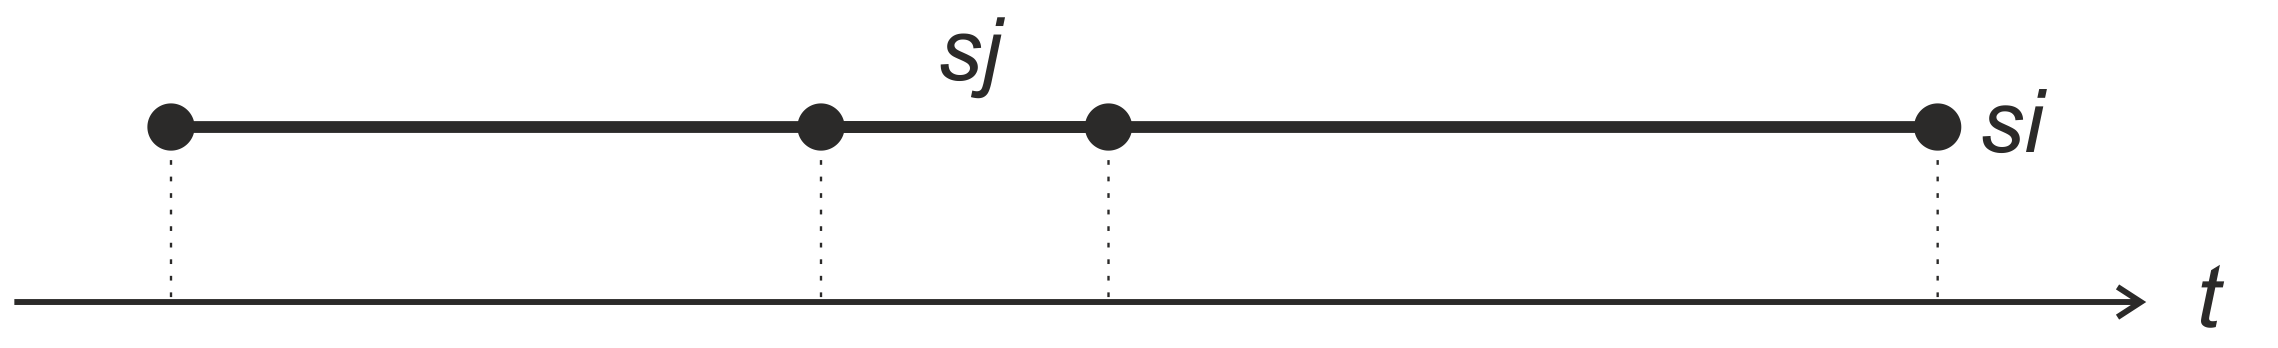
\includegraphics[width=1\linewidth]{figures/sd_temp_entities/img_temporal_part.png}}}
\scntext{примечание}{Связки отношения \textbf{\textit{темпоральная часть*}} связывают две \textit{временные сущности}, одна из которых является частью другой, например, действие и одно из его поддействий. Соответственно, период существования одной из этих сущностей всегда будет включаться в период существования другой (большей).

В отличие от более общего отношения \textit{темпоральное включение*}, связки которого могут связывать любые \textit{временные сущности}, связки отношения \textbf{\textit{темпоральная часть*}} связывают только \textit{временные сущности}, одна из которых является частью другой.}

\scnheader{следует отличать*}
\scnhaselementset{темпоральная часть*\\
	\scnaddlevel{1}
		\scnsuperset{подпроцесс*}
	\scnaddlevel{-1}
	;темпоральное включение*\\
\scnaddlevel{1}
	\scnnote{Связь \textit{темпорального включения*} может связывать абсолютно разные \textit{временные сущности}, существующие в общем случае в разных местах, а не только \textit{временные сущности}, одна из которых является частью другой. Хотя формально и можно объединить любые разные \textit{временные сущности} в одну общую \textit{временную сущность}, далеко не всегда имеет смысл это делать.}
\scnaddlevel{-1}}

\scnheader{темпоральное включение без совпадения начальных и конечных моментов*}
\scnidtf{строгое темпоральное включение*}
\scnrelfrom{описание примера}{
\scnfilescg{figures/sd_temp_entities/strict_temporal_inclusion.png}}
\scnrelfrom{иллюстрация}{
\scnfileimage{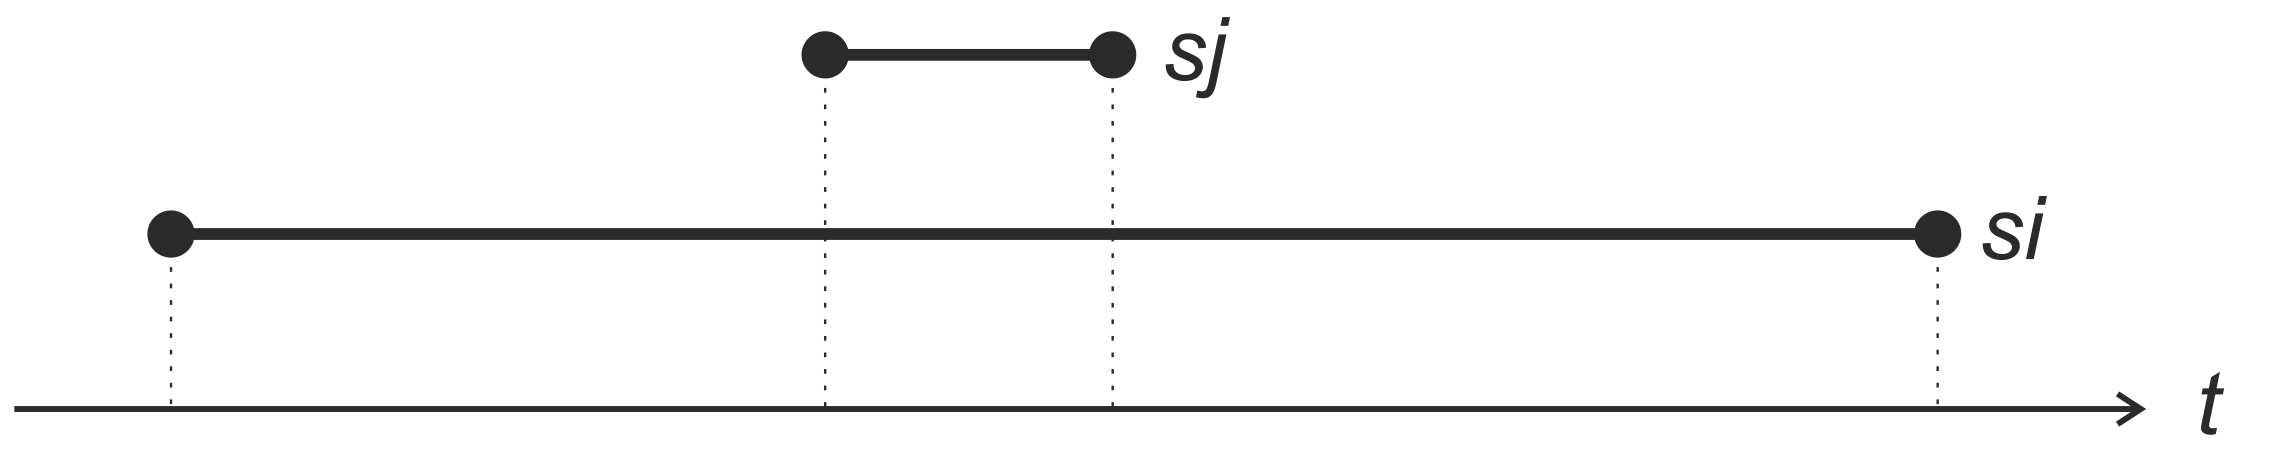
\includegraphics[width=1\linewidth]{figures/sd_temp_entities/img_strict_temporal_inclusion.png}}}

\scnheader{темпоральное включение с совпадением начальных моментов*}
\scnrelfrom{описание примера}{
\scnfilescg{figures/sd_temp_entities/temporal_include_with_match_start_points.png}}
\scnrelfrom{иллюстрация}{
\scnfileimage{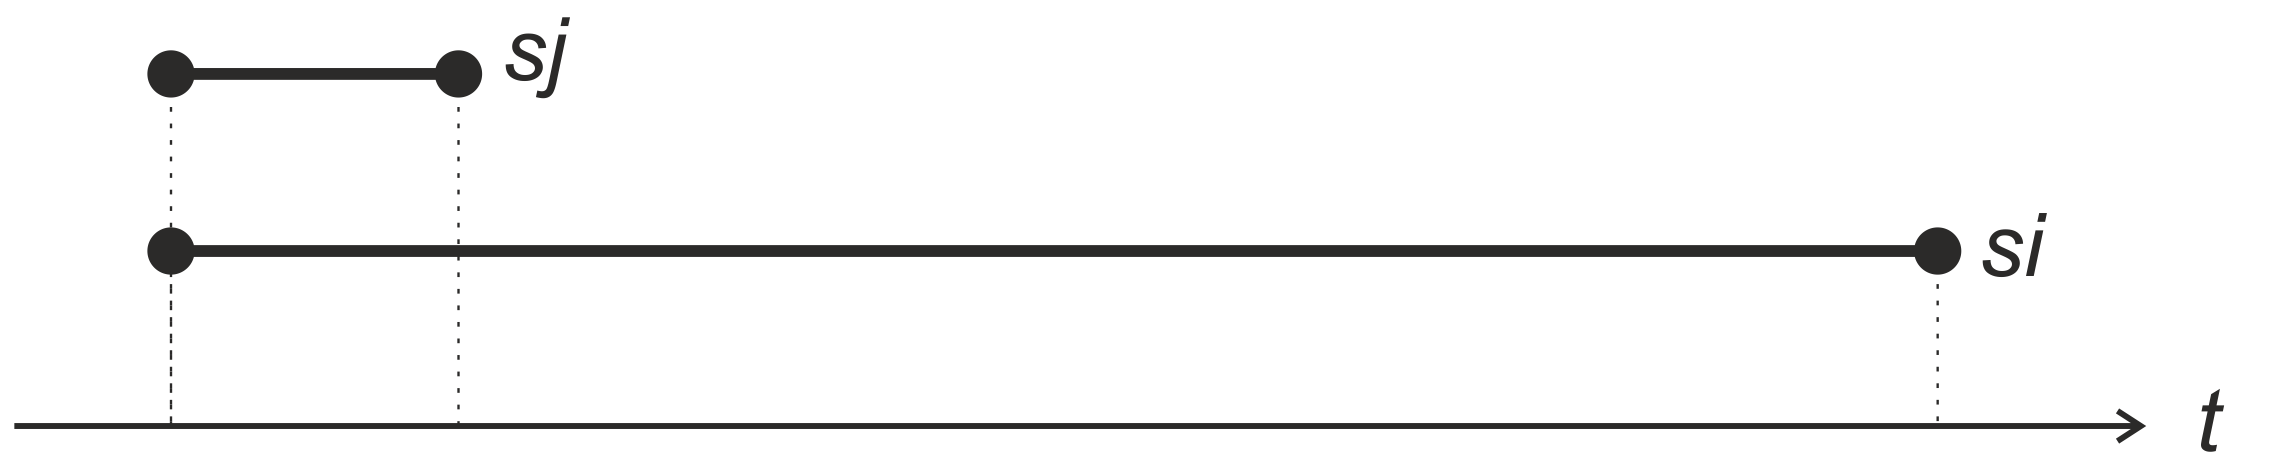
\includegraphics[width=1\linewidth]{figures/sd_temp_entities/img_temporal_include_with_match_start_points.png}}}

\scnheader{темпоральное включение с совпадением конечных моментов*}
\scnrelfrom{описание примера}{
\scnfilescg{figures/sd_temp_entities/temporal_include_with_terminal_point_match.png}}
\scnrelfrom{иллюстрация}{
\scnfileimage{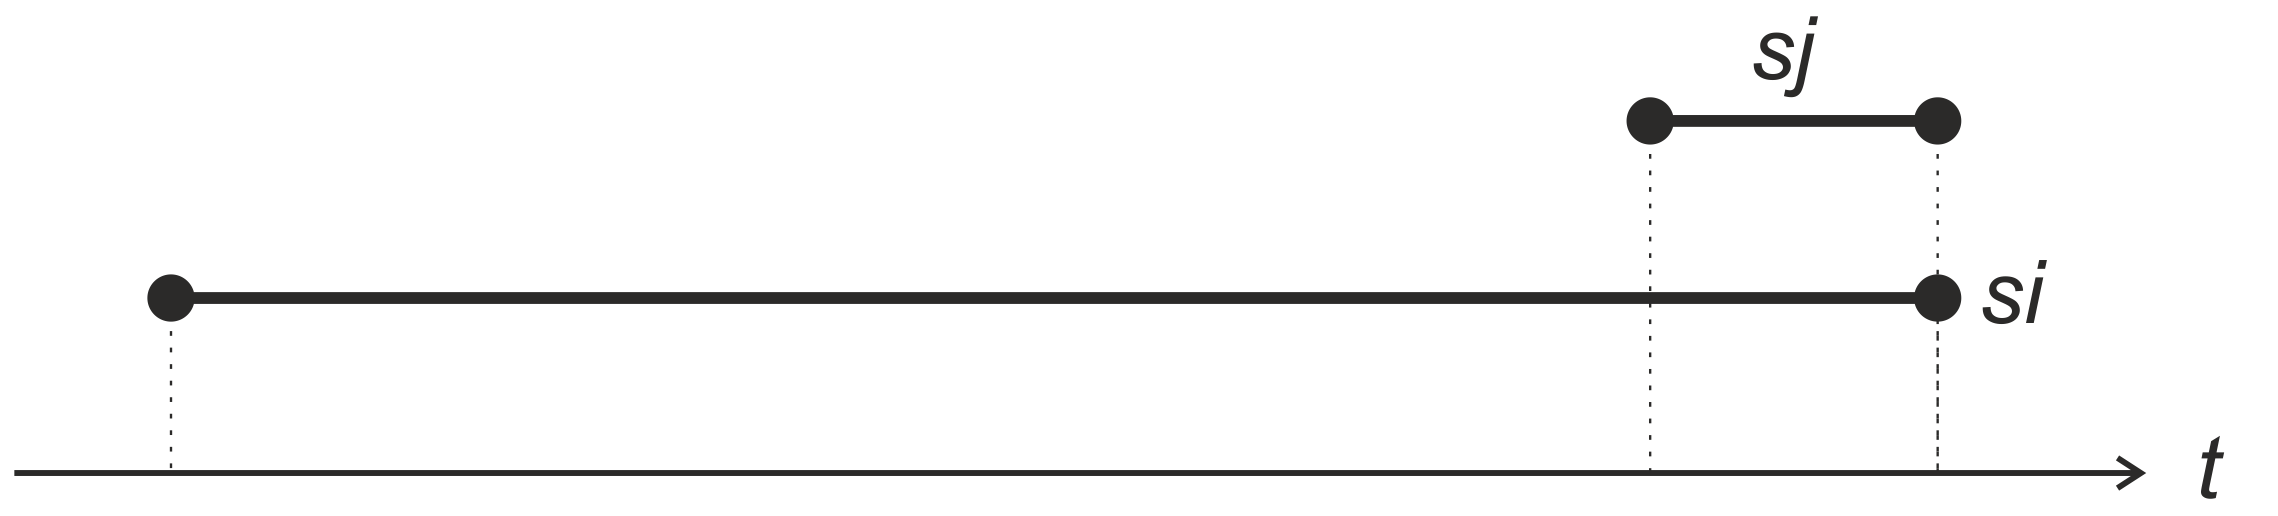
\includegraphics[width=1\linewidth]{figures/sd_temp_entities/img_temporal_include_with_terminal_point_match.png}}}

\scnheader{темпоральное совпадение*}
\scnidtf{совпадение начала и завершения*}
\scniselement{отношение эквивалентности}

\scnheader{темпоральное объединение*}
\scnidtf{преобразование нескольких временных сущностей в одну общую временную сущность, которая может оказаться прерывистой или даже дискретной*}
\scnrelboth{аналог}{объединение множеств*}
\scnnote{С формальной точки зрения объединять можно любые временные сущности. Но делать это надо только тогда, когда это имеет смысл, точно так же, как и в случае объединения множеств.}
\scnrelfrom{описание примера}{
\scnfilescg{figures/sd_temp_entities/temporal_union.png}}
\scnrelfrom{иллюстрация}{
\scnfileimage{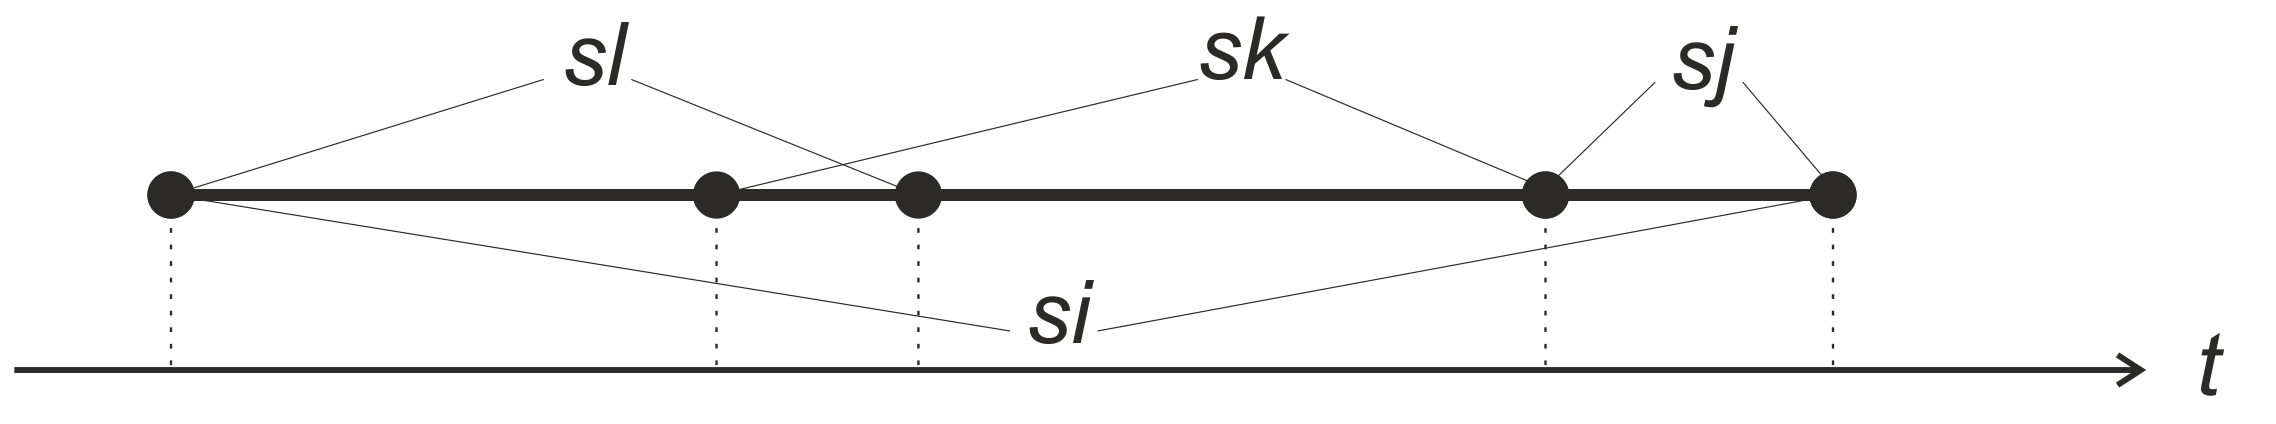
\includegraphics[width=1\linewidth]{figures/sd_temp_entities/img_temporal_union.png}}}

\scnheader{темпоральная декомпозиция*}
\scnidtf{Темпоральное отношение, связывающее временную сущность и множество смежных во времени временных сущностей, которые являются темпоральными частями исходной сущности и результатом темпорального объединения которых является исходная сущность*}
\scnrelboth{аналог}{разбиение*}
\scnrelfrom{описание примера}{
\scnfilescg{figures/sd_temp_entities/temporal_decomposition.png}}
\scnrelfrom{иллюстрация}{
\scnfileimage{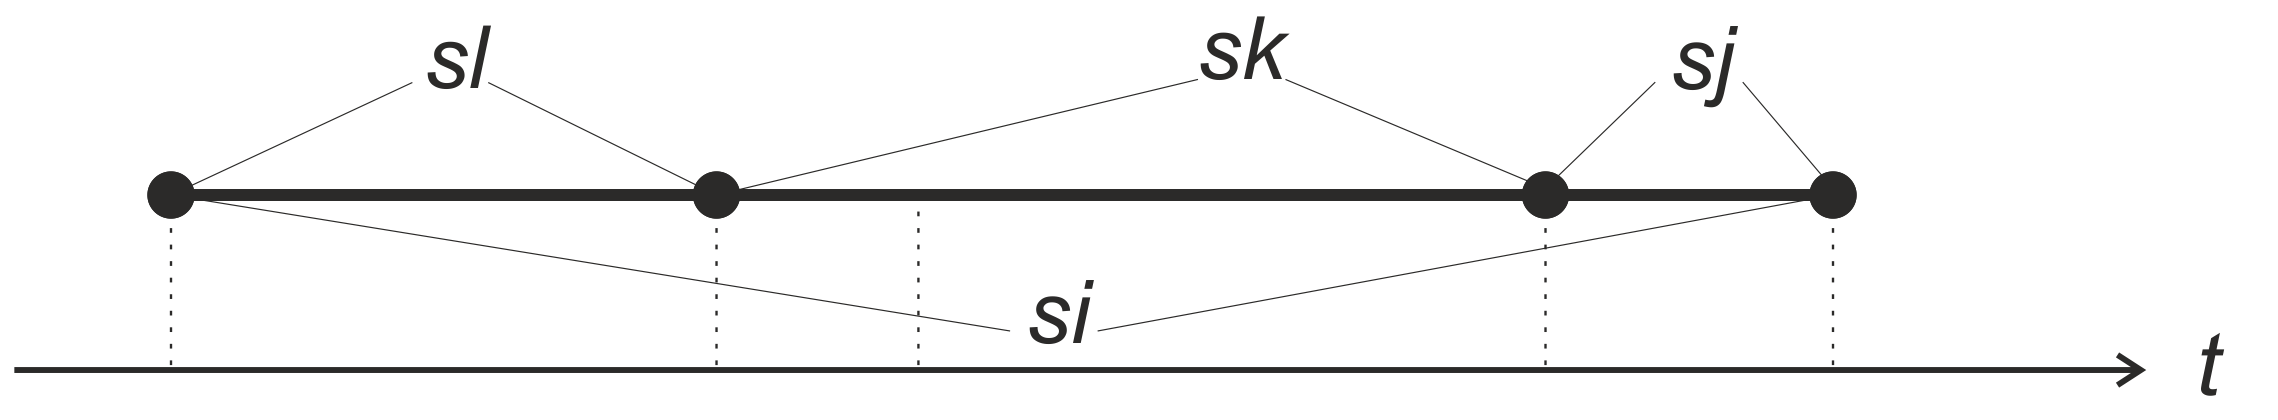
\includegraphics[width=1\linewidth]{figures/sd_temp_entities/img_temporal_decomposition.png}
}}

\scnheader{темпоральная смежность*}
\scnidtf{сразу позже*}
\scnidtf{смежность во времени*}
\scnidtf{строгая темпоральная последовательность (без темпорального промежутка)*}
\scnidtf{темпоральная последовательность без промежутка*}
\scnrelfrom{описание примера}{
\scnfilescg{figures/sd_temp_entities/temporal_adjacency.png}}
\scnrelfrom{иллюстрация}{
\scnfileimage{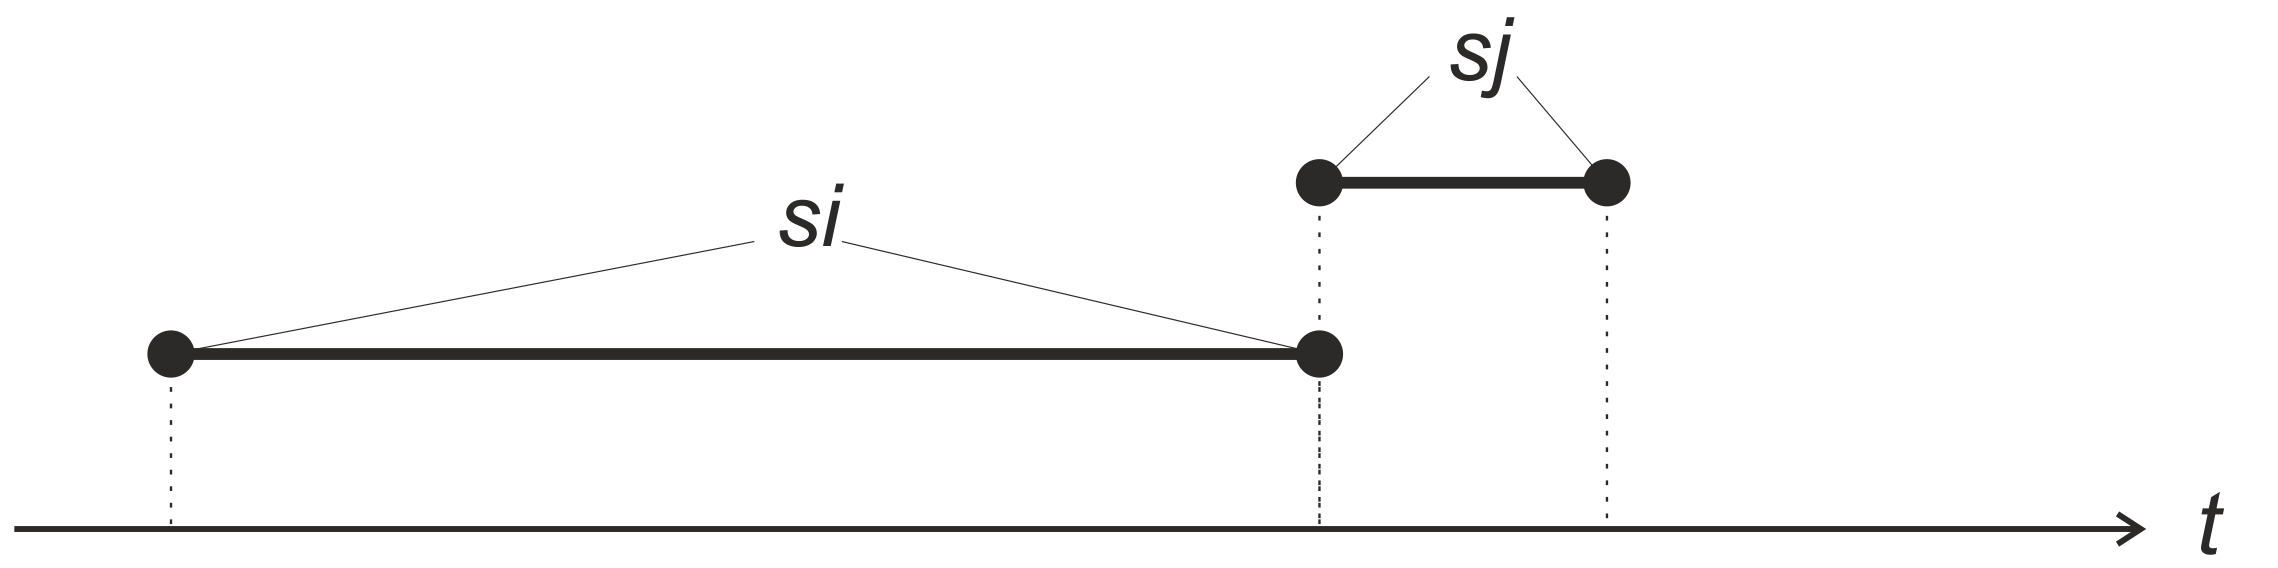
\includegraphics[width=1\linewidth]{figures/sd_temp_entities/img_temporal_adjacency.png}
}}

\scnheader{темпоральная последовательность с промежутком*}
\scnidtf{позже*}
\scnrelfrom{описание примера}{
\scnfilescg{figures/sd_temp_entities/temporal_sequence_with_intermediate.png}}
\scnrelfrom{иллюстрация}{
\scnfileimage{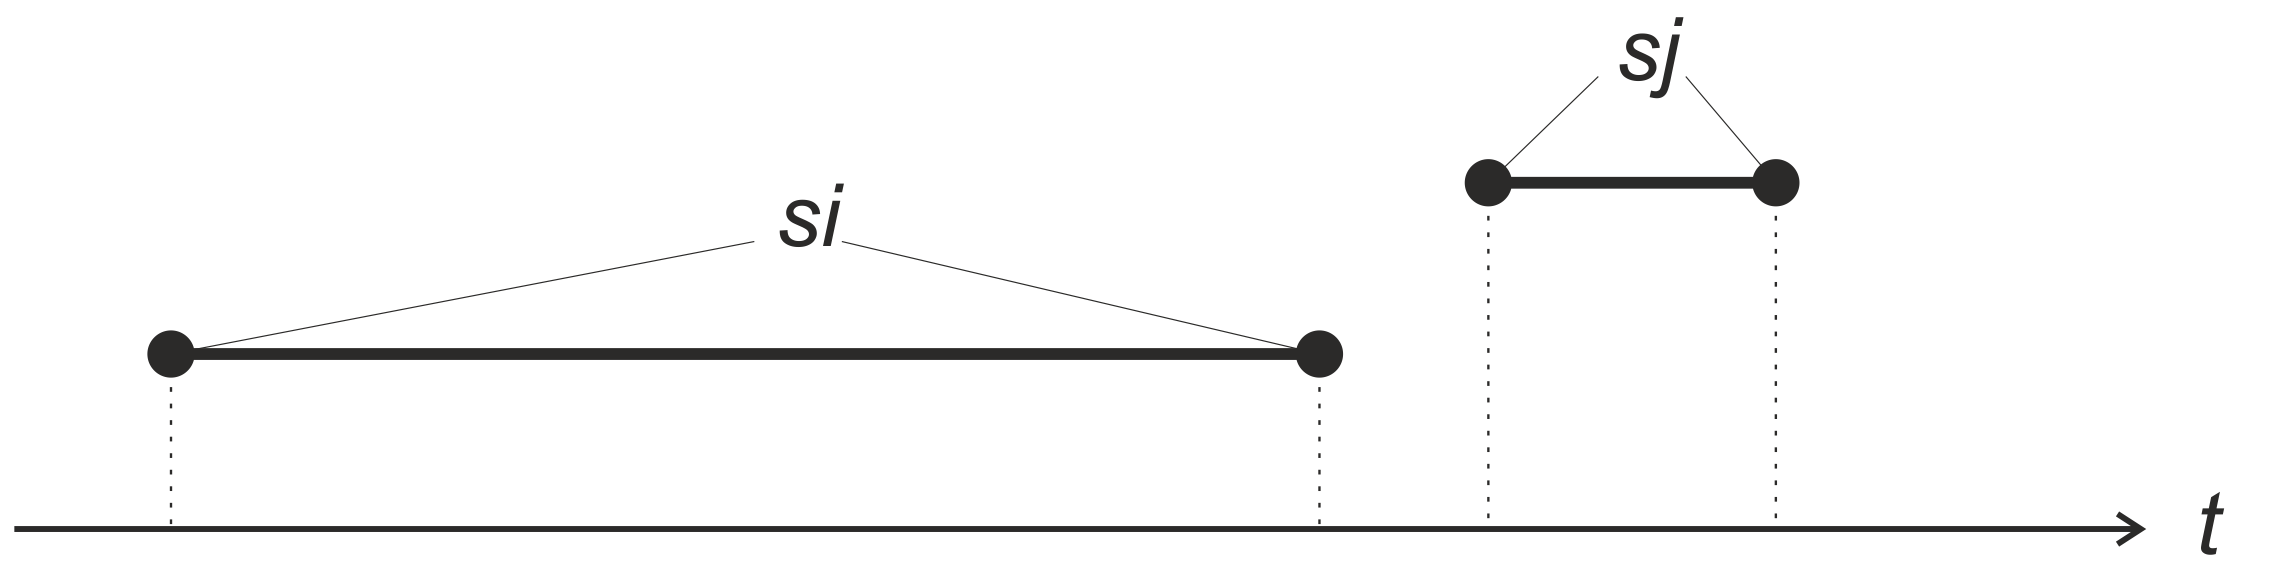
\includegraphics[width=1\linewidth]{figures/sd_temp_entities/img_temporal_sequence_with_intermediate.png}}}

\scnheader{темпоральная последовательность с пересечением*}
\scnrelfrom{описание примера}{
\scnfilescg{figures/sd_temp_entities/temporal_sequence_with_intersection.png}
}
\scnrelfrom{иллюстрация}{
\scnfileimage{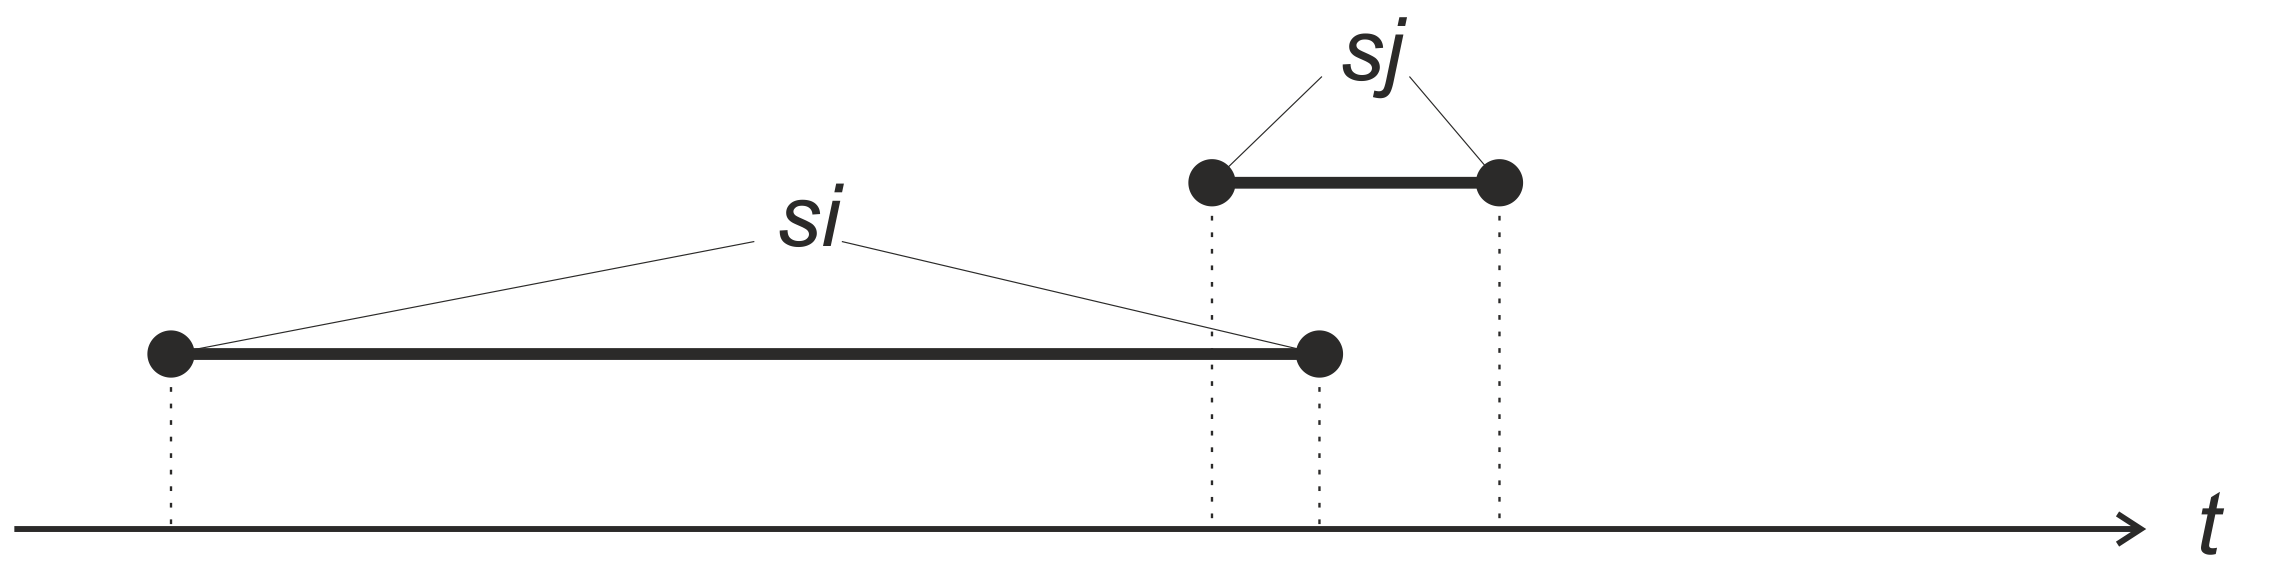
\includegraphics[width=1\linewidth]{figures/sd_temp_entities/img_temporal_cross_sequence.png}
}}

\scnheader{начало\scnsupergroupsign}
\scnidtf{одновременность начинаний\scnsupergroupsign}
\scnidtf{класс одновременно начавшихся сущностей\scnsupergroupsign}
\scniselement{параметр}
\scnexplanation{Каждый элемент множества \textbf{начало} представляет собой класс \textit{временных сущностей}, у которых совпадает момент начала их существования. Конкретное значение данного \textit{параметра} может быть как \textit{точной величиной}, так и \textit{неточной величиной} или \textit{интервальной величиной}.}
\scnrelfrom{описание примера}{
\scnfilescg{figures/sd_temp_entities/start.png}}
\scnaddlevel{1}
\scnexplanation{В данном примере \textbf{\textbf{\textit{ki}}} обозначает класс сущностей, начавших свое существование 19 февраля 2015 года по григорианскому календарю. Конкретные примеры таких сущностей -- \textbf{\textit{bi}} и \textbf{\textit{bj}}. \textbf{\textit{ti}} обозначает временную точку григорианского календаря, соответствующую 19 февраля 2015 года.}
\scnaddlevel{-1}

\scnheader{завершение\scnsupergroupsign}
\scnidtf{конец\scnsupergroupsign}
\scnidtf{одновременность завершений\scnsupergroupsign}
\scnidtf{класс одновременно завершившихся сущностей\scnsupergroupsign}
\scniselement{параметр}
\scnexplanation{Каждый элемент множества \textbf{\textit{завершение}} представляет собой класс \textit{временных сущностей}, у которых совпадает конечный момент их существования (момент завершения существования). Конкретное значение данного \textit{параметра} может быть как \textit{точной величиной}, так и \textit{неточной величиной} или \textit{интервальной величиной}.}
\scnrelfrom{описание примера}{
\scnfilescg{figures/sd_temp_entities/completion.png}}
\scnaddlevel{1}
\scnexplanation{В данном примере \textbf{\textit{ki}} обозначает класс сущностей, завершивших свое существование 21 февраля 2015 года по григорианскому календарю. Конкретные примеры таких сущностей -- \textbf{\textit{bi}} и \textbf{\textit{bj}}. \textbf{\textit{ti}} обозначает временную точку григорианского календаря, соответствующую 21 февраля 2015 года.}
\scnaddlevel{-1}

\scnheader{одновременность\scnsupergroupsign}
\scnidtf{параметр, значениями (элементами) которого являются классы либо одновременно существующих (происходящих) \textit{точечных временных сущностей}, одновременность которых рассматривается с заданной степенью точности, либо одновременно начинающихся и заканчивающихся длительных процессов}
\scnexplanation{Важно отметить, что элементами некоторого значения параметра \textit{одновременности} с заданной точностью могут быть только те временные сущности, которые и начались, и завершились в течение периода времени, заданного указанным значением этого параметра, но при этом начало и завершение этих временных сущностей не обязательно должно совпадать с началом и завершением указанного периода времени. Так, например, можно ввести значение параметра \textit{одновременности} ``\textit{2022 год по Григорианскому календарю}'', элементами которого будут все временные сущности, начавшие и закончившие свое существовавшие в рамках 2022 года. При этом не обязательно, чтобы эти временные сущности начались именно в полночь 1 января 2022 года и закончились в полночь 1 января 2023 года, это могут быть временные сущности, существовавшие, например, в течение июля 2022 года.}
\scnrelfrom{описание примера}{
\textit{}\scnfilescg{figures/sd_temp_entities/simultaneity.png}}
\scnaddlevel{1}
	\scnnote{Некоторые значения параметра одновременности могут быть подмножествами других значений того же параметра. Семантика такой связи будет выражаться в том, что первое из указанных значений описывает \textit{одновременность} \textit{временных сущностей} с большей точностью. Так, в приведенном примере величина ``\textit{2002 год}'' описывает одновременность временных сущностей с точностью до года, а величина ``\textit{июль 2022 года}'' описывает одновременность временных сущностей с точностью до месяца. При этом очевидно, что сущности, входящие во величину ``\textit{июль 2022 года}'' будут также входить и в величину ``\textit{2022 год}'' (как например временная сущность $\bm{sk})$. В приведенном примере для простоты предполагается, что все измерения производятся по Григорианскому календарю.}
\scnaddlevel{-1}

\scnheader{соединение значений ориентированного параметра*}
\scnrelfrom{описание примера}{
	\scnfilescg{figures/sd_temp_entities/temporal_values_join.png}
}
\scnaddlevel{1}
\scnnote{В приведенном примере множество сущностей, существовавших 10.01.2022, и множество сущностей, существовавших 12.01.2022, при помощи отношения \textit{соединение значений ориентированного параметра*} образуют множество сущностей, существовавших в период 10-12.02.2022.}
\scnaddlevel{-1}

\scnheader{следует отличать*}
\scnhaselementset{темпоральное совпадение*\\
	\scnaddlevel{1}
		\scniselement{отношение эквивалентности}
	\scnaddlevel{-1}
	;одновременность\scnsupergroupsign\\
	\scnaddlevel{1}
		\scnidtf{фактор-множество для отношения темпоральное совпадение*}
	\scnaddlevel{-1}}

\scnheader{длительность\scnsupergroupsign}
\scnidtf{класс временных сущностей, имеющих одинаковую длительность\scnsupergroupsign}
\scniselement{параметр}
\scnhaselement{тысячелетие}
\scnhaselement{век}
\scnhaselement{год}
\scnhaselement{месяц}
\scnhaselement{день}
\scnhaselement{час}
\scnhaselement{минута}
\scnhaselement{секунда}
\scnexplanation{Каждый элемент множества \textbf{\textit{длительность}} представляет собой класс \textit{временных сущностей}, у которых совпадает длительность их существования. Конкретное значение данного \textit{параметра} может быть как \textit{точной величиной}, так и \textit{неточной величиной} или \textit{интервальной величиной}.}
\scnrelfrom{описание примера}{
\scnfilescg{figures/sd_temp_entities/duration.png}}
\scnaddlevel{1}
\scnexplanation{В данном примере \textbf{\textit{ki}} обозначает класс сущностей, существовавших в течение 2 месяцев. Конкретный пример такой сущности -- \textbf{\textit{bi}}.}
\scnaddlevel{-1}

\bigskip
\scnendstruct \scnendcurrentsectioncomment

\end{SCn}